\documentclass[a4paper,12pt]{report}

\RequirePackage[french]{babel} %Langue du document
\RequirePackage[utf8]{inputenc} %Caractères spéciaux
\RequirePackage[section]{placeins}%Pour placement de section
\RequirePackage[T1]{fontenc} %Quelques lettres qui sont pas inclus dans UTF-8
\RequirePackage{mathtools} %Paquet pour des équations et symboles mathématiques
\RequirePackage{siunitx} %Pour écrire avec la notation scientifique (Ex.: \num{2e+9})
\RequirePackage{float} %Pour placement d'images
\RequirePackage{graphicx} %Paquet pour insérer des images
\RequirePackage[justification=centering]{caption} %Pour les légendes centralisées
\RequirePackage{subcaption}
\RequirePackage{wallpaper}
\RequirePackage{nomencl}
%\makenomenclature
\RequirePackage{fancyhdr}
%\pagestyle{fancy}
%\fancyheadoffset{1cm}
%\setlength{\headheight}{2cm}
\RequirePackage{url}
\RequirePackage[hidelinks]{hyperref}%Paquet pour insérer légendes dans des sous-figures comme Figure 1a, 1b
\RequirePackage[left=2.5cm,right=2.5cm,top=2cm,bottom=3.5cm]{geometry} %Configuration de la page
\RequirePackage{changepage}
\RequirePackage{url}
\RequirePackage{pdftricks2}
\RequirePackage{enumitem}
\RequirePackage[retainorgcmds]{IEEEtrantools}
\numberwithin{equation}{section}
\RequirePackage{xcolor}
\RequirePackage{amsfonts}
\usepackage{graphicx}
\usepackage{wrapfig}
\usepackage{lscape}
\usepackage{rotating}
\usepackage{epstopdf}
\usepackage{afterpage}
\usepackage{supertabular}


\begin{document}

\makenomenclature
\pagestyle{fancy}
\fancyheadoffset{1cm}
\setlength{\headheight}{2cm}
\lhead{
\includegraphics[scale=0.3]{um5.png}} %Affichage de l'image au top de la page
\rhead{
\includegraphics[scale=0.2]{ENSIAS.png}}

\begin{titlepage}
    \changepage{2cm}%amount added to textheight
               {}%amount added to textwidth
               {}%amount added to evensidemargin
               {}%amount added to oddsidemargin
               {}%amount added to columnsep
               {-2cm}%amount added to topmargin
               {}%amount added to headheight
               {}%amount added to headsep
               {}%amount added to footskip
    
    \setlength{\wpYoffset}{-7cm}    
    \ThisCenterWallPaper{0.4}{logo.png}
        \flushleft
        
\includegraphics[width=0.27\textwidth]{um5.png} %Insertion du logo
        \hfill
        
\includegraphics[width=0.20\textwidth]{ENSIAS.png}\par\vspace{1cm}
        \centering 
        {\scshape\LARGE Ecole Nationale Supérieure d'Informatique et d'Analyse des Systèmes \par Université Mohammed V  \par} %Nom de l'université
        \vspace{1.5cm}%Espace de 1,5cm
        {\scshape\Large Génie Logiciel \\ Projet de fin de deuxième année	\par} %sous-titre
        \vspace{1cm}%Espace de 1cm
        \rule{\linewidth}{0.2 mm} \\[0.4 cm]
        {\huge\bfseries Simulateur de calcul des prix des transactions immobilières \par} \
        \rule{\linewidth}{0.2 mm} \\[1.5 cm]
        \vspace{3cm}%Espace de 3cm
        
        \begin{minipage}{0.5\textwidth} %Minipage pour faire deux colonnes
            \begin{flushleft} \large %Envoyer à gauche
            \emph{\textbf{Réalisé par :}}\\ %Pour le titre au dessus des noms à gauche
            Tarmoune Oussama\\Serroukh Anass
            \end{flushleft}
        \end{minipage}
        ~
        \begin{minipage}{0.4\textwidth}
            \begin{flushright} \large
             \emph{\textbf{Encadré par :}} \\
             W.Ettazi \\
            \end{flushright}
        \end{minipage}\\[1cm]
        
        \vfill
        {\large \today\par} %Affichage de la date
    
\end{titlepage}

\tableofcontents
\vspace{1cm}
\listoffigures
\newpage
\listoftables
\newpage

\vspace*{7cm}
\begin{center}
    {\huge\bfseries Remerciements\par} \
\end{center}
{\large \par Nous tenons à exprimer notre profonde gratitude à notre professeur encadrante, 
Pr \textbf{Widad Ettazi}, pour son soutien constant et ses conseils avisés tout au long de ce projet. 
Votre expertise et votre disponibilité ont été des éléments clés dans la réussite de ce travail. 
Votre capacité à nous guider à travers les défis techniques et méthodologiques a été inestimable, 
et votre engagement envers notre réussite a été une source de motivation continue.\par}
\newpage

\vspace*{6cm}
\begin{center}
    {\huge\bfseries Résumé\par} \
\end{center}
{\large  \par Le projet \textbf{Simulateur de Calcul des Prix des Transactions Immobilières} vise à fournir 
une solution fiable et pratique pour estimer les prix de vente ou de location de biens immobiliers 
au Maroc. En raison du caractère privé des données immobilières dans le pays, nous avons opté pour 
le web scraping des sites d'annonces pour collecter les informations nécessaires. Après avoir nettoyé
 et structuré ces données, nous avons développé une application web permettant aux utilisateurs 
 d'effectuer des estimations précises et de recevoir des notifications sur les évolutions des prix. 
Le site propose également un tableau de bord pour les administrateurs afin de surveiller et gérer 
les opérations du système.\par}
\newpage


\vspace*{5.5cm}
\begin{center}
    {\huge\bfseries Abstract\par} \
\end{center}
{\large  \par \textbf{Real Estate Transaction Price Simulation} project aims to provide a reliable and 
practical solution for estimating the sale or rental prices of real estate properties in Morocco. 
Given the private nature of real estate data in the country, we utilized web scraping techniques 
to gather necessary information from real estate listing websites. Following data collection, we 
implemented a thorough data cleaning process to ensure accuracy and reliability. The project 
culminated in the development of a web application that allows users to perform precise estimations
 and receive notifications about price changes. Additionally, the platform includes an administrative
  dashboard for monitoring and managing system operations. This project demonstrates the effective 
  use of data scraping, cleaning, and modeling to deliver a valuable tool for the real estate 
  market.\par}

\newpage


\vspace*{3.5cm}
\begin{center}
    {\huge\bfseries Mots clé\par} \
\end{center}
{\large Immobilier, Estimation de Prix, Web Scraping, Nettoyage de Données, Modélisation de Données, MongoDB, Maroc, Annonces Immobilières, Système de Notifications, Tableau de Bord Administratif.\par}

\vspace*{3.5cm}
\begin{center}
    {\huge\bfseries Keywords\par} \
\end{center}
{\large Real Estate, Price Estimation, Web Scraping, Data Cleaning, Data Modeling, MongoDB, Morocco, Real Estate Listings, Notification System, Administrative Dashboard.\par}


\newpage

\vspace*{3cm}
\begin{center}
    {\huge\bfseries Introduction\par} \
\end{center}
{\large  
\par Le marché immobilier au Maroc est en constante évolution, avec des prix de vente et de location fluctuants en fonction de divers facteurs économiques et géographiques. Cependant, l'accès à des données précises et actuelles sur les prix immobiliers reste un défi majeur, en raison de la nature privée de ces informations. Le projet \textbf{Simulateur de Calcul des Prix des Transactions Immobilières} a été conçu pour pallier cette lacune en fournissant un outil fiable permettant d'estimer les prix des biens immobiliers à partir de données réelles collectées en ligne. 
\par Pour atteindre cet objectif, nous avons adopté une approche basée sur le web scraping, en ciblant les sites d'annonces immobilières tels qu'\url{avito.ma}. Cette méthode nous a permis de recueillir des données détaillées sur les propriétés, telles que les appartements, maisons, villas, bureaux et locaux commerciaux, selon les villes et le type de transaction (vente ou location). Ces données ont ensuite été nettoyées et structurées pour assurer leur précision et leur pertinence, permettant ainsi de développer une application web robuste offrant des estimations précises, des notifications sur les évolutions de prix, et un tableau de bord administratif pour la gestion des opérations.\par}


\newpage
%Chapter 1
\chapter{Contexte et Objectfs}
\section{Contexte général}
\vspace{0.5cm}
{\large
\par Le secteur immobilier joue un rôle crucial dans l'économie marocaine, représentant une part significative du PIB et influençant divers autres secteurs économiques. Toutefois, le marché immobilier marocain est caractérisé par un manque de transparence et d'accessibilité des données, ce qui complique la prise de décision pour les acheteurs, les vendeurs et les investisseurs. Les informations sur les prix des biens immobiliers sont souvent difficiles à obtenir, et les estimations disponibles peuvent varier considérablement, rendant la prévision des tendances du marché un défi de taille. \par
}
\vspace{0.5cm}
\section{Problématique}
\vspace{0.5cm}
{\large
\par La principale problématique dans le contexte du marché immobilier marocain réside dans l'accès limité à des données fiables et actuelles sur les prix des biens immobiliers. Cette absence de transparence crée une incertitude pour les acteurs du marché, qu'il s'agisse de particuliers souhaitant acheter ou vendre un bien, ou d'investisseurs cherchant à évaluer la rentabilité de leurs investissements. Les informations disponibles sont souvent fragmentées, obsolètes ou difficiles à comparer, ce qui rend la prise de décision complexe et risquée. De plus, les méthodes traditionnelles d'estimation des prix ne parviennent pas toujours à refléter les réalités du marché local, notamment en raison des variations régionales et des spécificités des biens immobiliers.\par
}
\newpage
\vspace*{2.5cm}
\section{Objectif}
\vspace{0.5cm}
{\large
\par Le projet \textbf{Simulateur de Calcul des Prix des Transactions Immobilières} a pour objectif de pallier cette problématique en développant une solution technologique capable de fournir des estimations de prix précises et fiables pour les biens immobiliers au Maroc. En utilisant des techniques avancées de web scraping, nous collectons des données détaillées et actualisées à partir de sites d'annonces immobilières. Ces données sont ensuite nettoyées, structurées et analysées pour offrir aux utilisateurs des estimations de prix basées sur des informations réelles et pertinentes. En plus de fournir des estimations, l'application propose des fonctionnalités telles que des notifications sur les évolutions de prix et un tableau de bord administratif pour la gestion et la surveillance des opérations. 
\par L'objectif final est de créer un outil accessible et utile pour tous les acteurs du marché immobilier, facilitant ainsi la prise de décision et renforçant la confiance dans les transactions immobilières.\par
}

\newpage
%Chapter 2
\chapter{Méthodologie de développement et Planning du projet}
\section{Méthodologie de développement}
\vspace{0.5cm}
{\large
\par Pour mener à bien le projet \textbf{Simulateur de Calcul des Prix des Transactions Immobilières}, nous avons adopté la méthodologie \textbf{Agile}. Cette approche itérative et flexible nous a permis de répondre de manière efficace aux exigences changeantes et d'améliorer continuellement le produit tout au long du cycle de développement. La méthodologie Agile se caractérise par des cycles de développement courts appelés "sprints", chacun d'une durée d'une semaine, au cours desquels des fonctionnalités spécifiques sont planifiées, développées, testées et évaluées.\par
}
\vspace*{0.5cm}
\begin{enumerate}
    \item \large{\textbf{Analyse des Besoins et Définition des Données}: Comprendre les exigences du projet et définir les types de données nécessaires pour fournir des estimations précises. }
    \item \large{\textbf{Collecte des Données via Web Scraping}: Récupérer les données nécessaires à partir des sites web d'annonces immobilières. }
    \item \large{\textbf{Nettoyage et Structuration des Données}: Assurer que les données collectées sont précises, complètes et utilisables.}
    \item \large{\textbf{Développement de l'Application Web}: Créer une interface utilisateur permettant d'accéder aux fonctionnalités d'estimation et de gestion des données.}
    \item \large{\textbf{Modélisation et Analyse des Données}: Développer des modèles capables de fournir des estimations précises et des analyses statistiques.}
    \item \large{\textbf{Déploiement et Automatisation}: Assurer que l'application est accessible et performante pour les utilisateurs finaux.}
    \item \large{\textbf{Tests et Validation}: Garantir la fiabilité et la performance de l'application avant son lancement. }
\end{enumerate}

\section{Planning du projet}
\vspace{0.5cm}
{\large
\par Le diagramme de Gantt ci-dessous illustre la répartition des sprints et le calendrier prévu pour la réalisation du projet.
}
\vspace{0.5cm}
\begin{figure}[h]
    \centering
        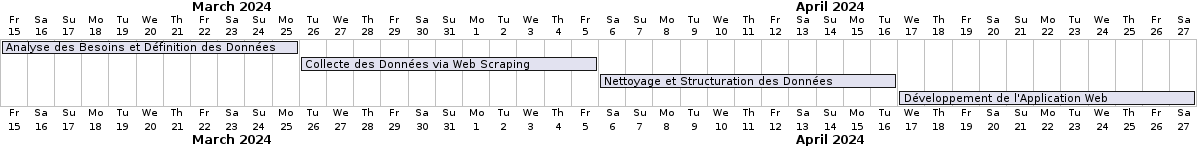
\includegraphics[width=\textwidth]{gantt1.png}
        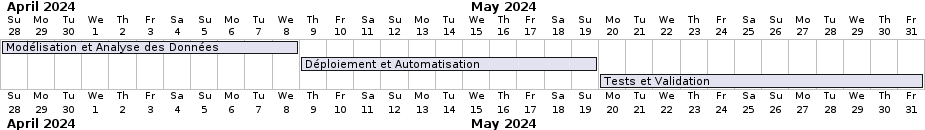
\includegraphics[width=\textwidth]{gantt2.png}
    \caption{Diagramme de Gantt}
\end{figure}



\newpage
%Chapter 3
\chapter{Le Web Scraping}
\section{Définition}
\vspace{0.5cm}
\large{
\par Le web scraping, également appelé extraction de données web, est une technique utilisée pour extraire des informations à partir de sites web. Cette méthode implique l'utilisation de logiciels ou de scripts pour parcourir et récupérer des données disponibles publiquement sur internet. Contrairement aux API, qui fournissent des données de manière structurée et contrôlée, le web scraping permet d'extraire des informations directement à partir des pages web, en imitant la navigation et l'interaction d'un utilisateur humain.\par
}
\section{Le Web Scraping dans notre Projet}
\vspace{0.5cm}
\large{
\par Dans le cadre de notre projet Simulateur de Calcul des Prix des Transactions Immobilières, le web scraping a été essentiel pour collecter les données nécessaires en raison du caractère privé des informations immobilières au Maroc. Nous avons ciblé les sites d'annonces immobilières, notamment avito.ma, pour extraire les données relatives aux biens immobiliers (appartements, maisons, villas, bureaux, locaux commerciaux) en fonction des villes et du type de transaction (vente ou location). Cette approche nous a permis de constituer une base de données riche et détaillée pour notre application.\par
}
\section{Benchmark des Outils de Scraping}
\vspace{0.5cm}
\large{
\par Pour réaliser le web scraping, plusieurs outils et frameworks sont disponibles. Nous avons effectué un benchmark des outils les plus populaires pour déterminer celui qui répondrait le mieux à nos besoins :\par
}
\vspace*{0.5cm}
\begin{enumerate}
    \item \large{\textbf{BeautifulSoup}: Une bibliothèque Python utilisée pour parser des documents HTML et XML. Elle est simple d'utilisation mais nécessite d'être combinée avec d'autres bibliothèques pour la gestion des requêtes HTTP. }
    \item \large{\textbf{Scrapy}: Un framework open-source en Python, spécialement conçu pour le web scraping. Il est très puissant et permet de gérer des projets de scraping complexes avec des fonctionnalités intégrées pour le crawling, le parsing, le stockage des données et la gestion des erreurs. }
    \item \large{\textbf{Selenium}: Un outil permettant d'automatiser les navigateurs web. Il est utile pour scraper des sites dynamiques générés par JavaScript, mais il est plus lent et plus lourd que les autres options.}
    \item \large{\textbf{Splash}: Un outil de rendu de pages web, capable d'exécuter JavaScript, qui peut être utilisé avec Scrapy pour scraper des sites dynamiques. Il offre une flexibilité pour gérer les pages complexes tout en restant intégré dans un environnement Scrapy.}
\end{enumerate}
\large{
\par Après avoir évalué ces options, nous avons opté pour Scrapy en combinaison avec Splash en raison de leur robustesse, de leur flexibilité et de leurs capacités avancées de gestion des projets de scraping.
}
\section{Méthodologie}
\large{
\par La méthodologie de web scraping que nous avons adoptée comprend les étapes suivantes :\par
}
\begin{enumerate}
    \item \textbf{Analyse des Sites Web Ciblés}
    \begin{itemize}
        \item[$\bullet$] Identification des sites web pertinents pour le projet.
        \item[$\bullet$] Analyse de la structure HTML des pages pour déterminer les éléments contenant les informations nécessaires (titres, prix, descriptions, localisations, etc.).
    \end{itemize}
    \item \textbf{Développement des Spiders}
    \begin{itemize}
        \item[$\bullet$] Création de spiders avec Scrapy pour automatiser la navigation et l'extraction des données.
        \item[$\bullet$] Intégration de Splash pour gérer les pages dynamiques et exécuter JavaScript.
        \item[$\bullet$] Implémentation de mécanismes pour contourner les blocages de bots, tels que l'utilisation de proxies et de délais aléatoires.
    \end{itemize}
    \item \textbf{Exécution et Collecte des Données}
    \begin{itemize}
        \item[$\bullet$] Exécution des spiders pour collecter les données brutes.
        \item[$\bullet$] Surveillance des performances et des erreurs lors de l'extraction.
    \end{itemize}
    \item \textbf{Nettoyage et Structuration des Données}
    \begin{itemize}
        \item[$\bullet$] Nettoyage des données pour éliminer les doublons, les annonces fausses et compléter les informations manquantes.
        \item[$\bullet$] Conversion et structuration des données pour les rendre utilisables dans notre application.
    \end{itemize}
    \item \textbf{Stockage des Données}
    \begin{itemize}
        \item[$\bullet$] Stockage des données collectées et nettoyées dans une base de données.
        \item[$\bullet$] Mise en place de procédures de sauvegarde et de gestion des données.
    \end{itemize}
\end{enumerate}
\large{
\par En suivant cette méthodologie, nous avons pu obtenir une base de données fiable et complète, essentielle pour le fonctionnement de notre simulateur de calcul des prix des transactions immobilières.\par
}

\newpage
\chapter{Analyse et Conception}
\section{Identification des Acteurs}
\vspace{0.5cm}
\begin{enumerate}
    \item \textbf{Utilisateurs Finaux}
    \begin{itemize}
        \item[$\bullet$] \textbf{Clients Gratuits}: Utilisateurs qui accèdent aux fonctionnalités de base pour effectuer des estimations simples et recevoir des notifications par défaut.
        \item[$\bullet$] \textbf{Clients Abonnés}: Utilisateurs payants ayant accès à des fonctionnalités avancées, incluant des estimations complexes, des notifications personnalisées, et des graphiques d'évolution des prix.
    \end{itemize}
    \item \textbf{Administrateurs}
    \begin{itemize}
        \item[$\bullet$] \textbf{Admin}: Utilisateurs responsables de la gestion et de la surveillance de l'application, y compris la gestion des utilisateurs, le contrôle de la fréquence de scraping .
    \end{itemize}
\end{enumerate}

\section{Besoins Fonctionnels}
\vspace{0.5cm}
\begin{enumerate}
    \item \textbf{Estimation de Prix}
    \begin{itemize}
        \item[$\bullet$] Permettre aux utilisateurs de saisir les caractéristiques d'un bien immobilier (type de bien, localisation, surface, nombre de pièces, etc.).
        \item[$\bullet$] Générer des estimations de prix de vente ou de location basées sur les données collectées et nettoyées.
    \end{itemize}
    \newpage
    \item \textbf{Notifications}
    \begin{itemize}
        \item[$\bullet$] Envoyer des notifications aux utilisateurs concernant les évolutions de prix des biens immobiliers similaires.
        \item[$\bullet$] Permettre aux utilisateurs abonnés de personnaliser leurs notifications selon leurs préférences.
    \end{itemize}
    \item \textbf{Tableau de Bord}
    \begin{itemize}
        \item[$\bullet$] Offrir un tableau de bord interactif pour les utilisateurs abonnés, affichant des graphiques et des indicateurs sur les tendances des prix.
        \item[$\bullet$] Fournir un tableau de bord administratif pour surveiller la performance du système, gérer les utilisateurs, et configurer la fréquence de scraping.
    \end{itemize}
    \item \textbf{Gestion des Utilisateurs}
    \begin{itemize}
        \item[$\bullet$] Permettre l'inscription et la gestion des comptes utilisateurs.
        \item[$\bullet$] Gérer les plans d'abonnement et les paiements .
    \end{itemize}
    \item \textbf{Automatisation }
    \begin{itemize}
        \item[$\bullet$] Automatiser le processus de scraping et de nettoyage des données.
    \end{itemize}
\end{enumerate}

\section{Besoins Non Fonctionnels}
\vspace{0.5cm}
\begin{enumerate}
    \item \textbf{Sécurité}
    \begin{itemize}
        \item[$\bullet$] Garantir la sécurité des données des utilisateurs, y compris la protection des informations personnelles et des données de paiement.
    \end{itemize}
    \item \textbf{Scalabilité}
    \begin{itemize}
        \item[$\bullet$] Concevoir l'application de manière à pouvoir évoluer pour gérer une augmentation du nombre d'utilisateurs et de données à traiter.
    \end{itemize}
    \item \textbf{Maintenance}
    \begin{itemize}
        \item[$\bullet$] Faciliter la maintenance et les mises à jour de l'application, avec une documentation complète et des procédures de sauvegarde régulières.
    \end{itemize}
\end{enumerate}

\newpage
\section{Diagramme de cas d'utilsation}
\vspace{0.5cm}
\begin{figure}[h]
    \centering
        
\includegraphics[width=\textwidth]{uml-client_gratuit.png}
    \caption{Diagramme de cas d'utilsation "Client Gratuit"}
\end{figure}
\newpage
\vspace*{3.5cm}
\begin{figure}[h]
    \centering
        
\includegraphics[width=\textwidth]{uml-Client_abonne.png}
    \caption{Diagramme de cas d'utilsation "Client Abonné"}
\end{figure}
\newpage
\vspace*{3.5cm}
\begin{figure}[h]
    \centering
        
\includegraphics[width=\textwidth]{uml-Admin.png}
    \caption{Diagramme de cas d'utilsation "Admin"}
\end{figure}
\newpage
\section{Diagramme d'activités}
\vspace*{1cm}
\begin{figure}[h]
    \centering
        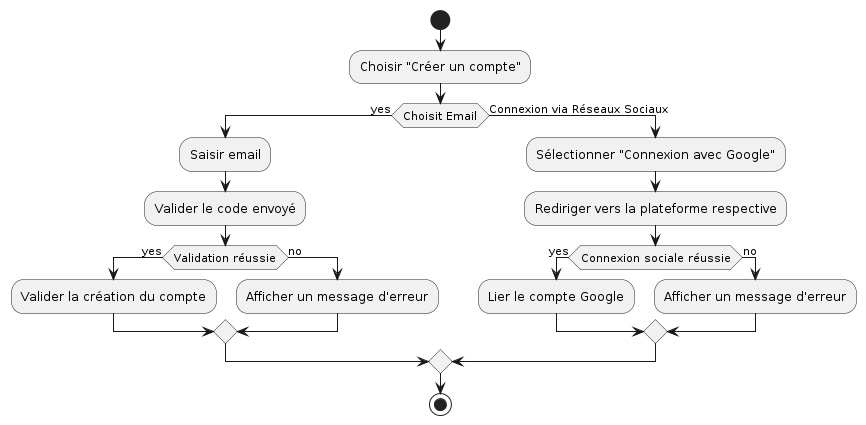
\includegraphics[width=\textwidth]{activity_account.png}
    \caption{activité de création du compte}
\end{figure}
\begin{figure}[h]
    \centering
        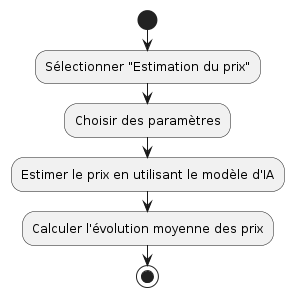
\includegraphics[width=0.5\textwidth]{activity_estimation.png}
    \caption{activité d’estimation du prix}
\end{figure}
\newpage
\section{Diagramme de classes}
\vspace{0.5cm}
\begin{figure}[h]
    \centering
        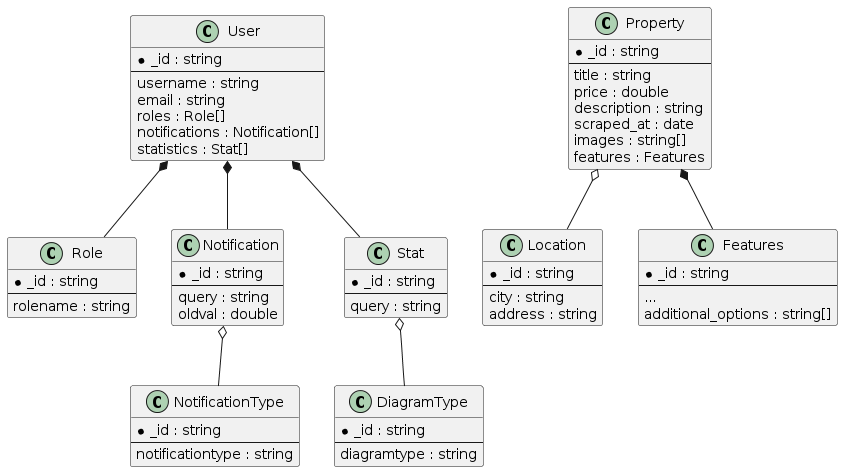
\includegraphics[width=\textwidth]{class.png}
    \caption{Diagramme de classes}
\end{figure}
\par Dans ce diagramme de classe, l'attribut \textit{\_id} de type string renvoie à la clé primaire générée automatiquement par \textbf{MongoDB}, le système de gestion de base de données utilisé par notre application. La classe User se distingue par ses identifiants, à l'exception du mot de passe, car nous utilisons un service dédié à l'authentification appelé \textbf{Kindle}. Les rôles sont définis par des désignations (client ou administrateur).
\\ \par
Les diagrammes sont catégorisés par leurs types (nuage de points, diagramme en barres, diagramme linéaire), ce qui détermine la manière dont les statistiques seront visualisées. Ces statistiques dépendent de divers critères de filtrage pour produire des indicateurs de performance clés (\textbf{KPI}), sauvegardés sous forme de requêtes \textbf{MongoDB}.
\\ \par
Les utilisateurs non abonnés peuvent obtenir des notifications simples en choisissant une fréquence de notification. En revanche, les utilisateurs abonnés peuvent obtenir des informations plus détaillées sur les annonces dans ces notifications.
\\ \par
Pour ce qui est des annonces, la classe Property représente la structure de leurs informations. Toutes ces propriétés partagent des attributs fondamentaux comme le titre, la description, et le prix. Les différences apparaissent lors du traitement de différents types de biens immobiliers ou de transactions. Cette fragmentation améliore les performances en éliminant la nécessité de filtrer les documents ou d'effectuer des jointures pour obtenir les annonces ciblées. Avec cinq types de biens immobiliers (appartements, maisons, villas, bureaux, locaux commerciaux) et deux types de transactions (location, vente), le nombre de classes peut devenir important. Il suffit donc de représenter les attributs partagés et de noter les différences entre ces classes. Ces variations sont présentées dans le tableau suivant :
\begin{table}[htbp]
    \centering
    \resizebox{\columnwidth}{!}{
    \begin{tabular}{|l|l|l|l|l|}
  \hline
  Appartement & Maisons & Villas & Bureaux & Locaux commerciaux \\
  \hline
  Age du bien & Age du bien & Age du bien & Num d'étage & Nbr de Salles de bain \\
  Nbr d'étages & Nbr d'étages & Nbr d'étages & Nbr de pièces &  \\
  Nbr de chambres & Nbr de chambres & Nbr de chambres & Nbr de Salles de bain &  \\
  Nbr de Salons & Nbr de Salons & Nbr de Salons &  &  \\
  Nbr de Salles de bain & Nbr de Salles de bain & Nbr de Salles de bain &  & \\
  \hline
  Balcon & Parking & Parking & Parking & Climatisation \\
  Ascenseur & Garage & Garage & Climatisation & Chauffage \\
  Terrasse & Balcon & Balcon & Chauffage & Sécurité \\
  Meublée & Terrasse & Terrasse & Sécurité & Parking \\
  Climatisation & Meublée & Meublée & Ascenseur & \\
  Chauffage & Climatisation & Climatisation & Terrasse & \\
  Cuisine équipée & Chauffage & Chauffage &  & \\
  Concierge & Cuisine équipée & Cuisine équipée &  & \\
  Sécurité & Jardin & Jardin &  & \\
  Parking & Sécurité & Sécurité &  & \\
  & Piscine & Piscine &  & \\
  \hline
\end{tabular}}
    \caption{tableau des attributs}
    \label{tab:tableau des attributs}
\end{table}
\vspace{1cm}
\par
La première ligne indique le type de bien immobilier, la deuxième énumère les attributs supplémentaires spécifiques à ce type, et la troisième liste les options additionnelles
associées à ce bien immobilier.
\newpage
\chapter{Réalisation du projet}
\section{Collecte, exploration, nettoyage et modélisation}
\par
Étant donné que les estimations des transactions immobilières requièrent des données de la réalité, nous avons décidé de collecter les informations à travers divers sites web marocains. 
\subsection{Collection de données : }
\par
La première étape a été de déterminer ces sites web en utilisant l'outil similarweb.com .Nous avons sélectionné le site avito.ma en raison de son classement élevé dans la catégorie "E-commerce \& Shopping", avec un nombre de visiteurs compris entre 2,1 et 2,2 millions. Ce site web était riche en annonces immobilières, tant pour la vente que la location.
\\ \par
La deuxième étape a consisté à déterminer les attributs à collecter pour chaque type d'immobilier. Nous avons créé des annonces sur chaque site afin de découvrir les champs à remplir, et vérifié leur existence via la fonctionnalité de recherche d'annonces.
\\ \par
Enfin, nous avons conçu un premier modèle simple pour enregistrer toutes les annonces, en appliquant des transformations sur les attributs pour harmoniser le format des données.Cette forme est spécifiée dans le tableau précédent au niveau du diagramme de classes.
\subsection{Exploration et nettoyage des données : }
\par
C'est souvent une tâche cruciale qui a un impact important sur la qualité et la fiabilité des analyses et des modèles ultérieurs. La gestion de données hétérogènes, la correction d'erreurs et d'incohérences, ainsi que la nécessité d'une expertise métier rendent le nettoyage des données difficile.
\\ \par
Les annonces dupliquées sont supprimées en se basant sur le lien comme critère. Cela ne couvre certainement pas le cas de plusieurs annonces différentes concernant la même propriété, mais nous supposons qu'elles sont négligeables.
\\ \par
Une remarque importante concerne l’analyse des attributs manquants.Nous essayons alors d’extraire les valeurs manquantes à partir de la description. Après des investigations sur de petits échantillons de données, nous remarquons que la description contient parfois des informations supplémentaires qui ne sont pas déjà mentionnées. Une grande partie de ces descriptions souffre d’erreurs orthographiques, d’incohérences, et parfois elles ne contiennent même pas de français. Néanmoins, Nous avons tenté d’utiliser la librairie spaCy pour une simple extraction des données. Cela commence par l'élimination des caractères irréguliers et des mots vides (stop words), et passe par la lemmatisation.
\\ \par
spaCy renvoie le noyau de dépendance d'un token à l'intérieur d'une phrase. Le noyau de dépendance représente le mot le plus important dont dépend le token courant sur le plan syntaxique. spaCy utilise l'analyse par dépendance pour examiner les relations entre les mots d'une phrase. Cependant, l’utilisation de cette technique pour rechercher les appellations des attributs (les mots-clés) s'est avérée insuffisante.
\\ \par
Nous sommes donc passés à l'API OpenAI pour la détermination des attributs manquants. Puisqu'elle utilise le grand modèle de langage ChatGPT, elle comprend automatiquement la description avec la structure du modèle. Nous utilisons cette API pour extraire des informations pertinentes et remplir ces champs. 
\\ \par
Les prix fluctuent entre des extrêmes irréalistes, c’est pourquoi nous utilisons une méthode de nettoyage des données basée sur les quartiles. Elle permet de nettoyer un ensemble de données en supprimant les valeurs aberrantes du prix. Cette technique s'appuie sur la détection des anomalies basées sur les quartiles, où les valeurs inférieures au 10e percentile et supérieures au 90e percentile sont considérées comme des anomalies et sont donc éliminées.
\par
Les valeurs de la colonne "ville" ont été converties en français pour les cas spéciaux contenant des mots en arabe.
\\ \par
Nous passons ainsi aux attributs particuliers à chaque type de propriété. Dans un premier temps, nous transformons ce dictionnaire en un tableau. À ce niveau, une grande partie des attributs est manquante. Nous observons les attributs booléens sous forme de liste et les transformons en plusieurs colonnes booléennes avec "True" signifiant la présence de l’option et vice-versa. Pour les attributs numériques avec des valeurs uniques et limitées (nombre de chambres, de salons, etc.), les valeurs sont bornées supérieurement (par exemple, avoir ‘7+’ chambres). Dans ce cas, il suffit d'en extraire le nombre.
\\ \par
La dernière transformation s’agit de remplacer le prix par le prix par mètre carré en divisant sur la surface.Les données collectées sont ensuite stockées dans la collection appropriée selon le type d’immobilier et la nature de la transaction.
\subsection{Le modèle d’estimation du prix}
\par 
En raison des règles de validation limitées des sites web sources, nous avons remarqué que certains attributs soi-disant numériques ne sont pas garantis d'être des nombres. Parfois, il s'agit d'intervalles ou de mots (comme dans le cas de l'âge de la propriété). Heureusement, cela concerne un ensemble limité de valeurs ordonnées que nous pouvons simplement remplacer par des nombres pour l'entraînement de l’IA.
\\ \par
Après avoir nettoyé les données, nous sommes finalement prêts à entraîner un modèle pour prédire ou estimer le prix, après avoir appliqué la technique du one-hot encoding. Nous avons choisi d’utiliser la forêt d'arbres décisionnels en raison de sa robustesse aux valeurs aberrantes et aux données non équilibrées, ainsi que de sa capacité à représenter les relations complexes. Malheureusement, elle s'est avérée incapable de prédire le prix avec une bonne précision (marge de 1000 dirhams).
\\ \par
Ensuite, nous avons utilisé la régression linéaire. Cette dernière permet de détecter les relations linéaires entre le prix et les autres attributs. Cette fois, le modèle s'est révélé performant en termes de précision et de rapidité, avec une marge inférieure à 20 dirhams.
\begin{figure}[H]
    \centering
    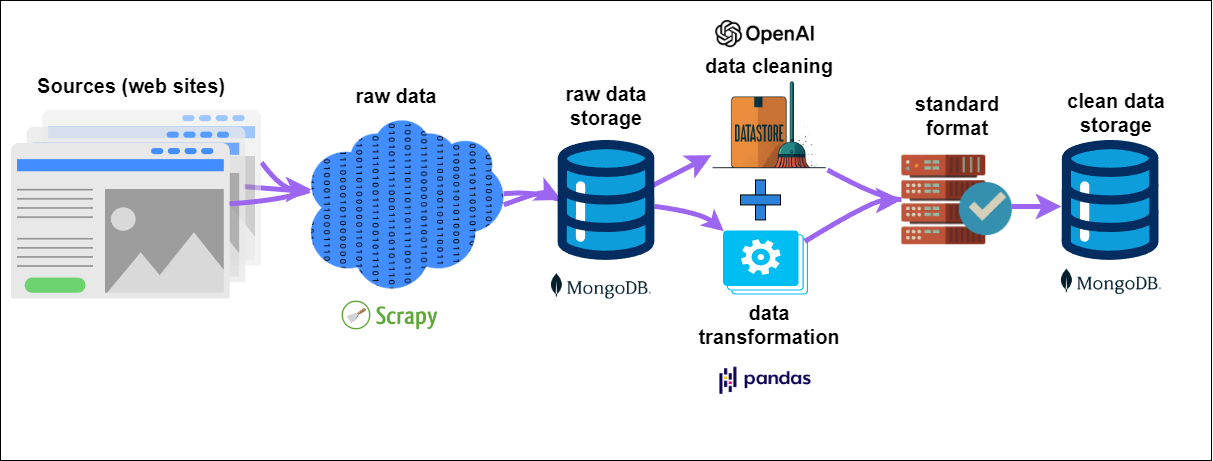
\includegraphics[width=\textwidth]{web-scrapping-architecture.png}
    \caption{data pipeline}
    \label{fig:data pipeline}
\end{figure}
\newpage
\section{Choix techniques}
\subsection{scrapy}
\begin{figure}[H]
    \centering
    
\includegraphics[width=0.5\textwidth]{tech/scrapy.png}
    \caption{scrapy logo}
    \label{fig:scrapy logo}
\end{figure}
\par
Scrapy est un framework open-source en Python conçu pour le web scraping, qui consiste à extraire automatiquement des données à partir de sites web. Il est apprécié pour sa flexibilité et sa puissance, permettant aux développeurs de créer des spiders ou crawlers complexes pour collecter des informations à grande échelle. Scrapy offre une structure bien organisée pour gérer les différentes étapes du web scraping, allant de la requête initiale aux transformations des données extraites.\\ \par
Le processus commence par la définition de spiders, qui sont des classes Python personnalisées. Ces spiders indiquent à Scrapy comment naviguer sur un site web spécifique et quels éléments HTML doivent être extraits. Grâce à Scrapy, les développeurs peuvent envoyer des requêtes HTTP, suivre les liens sur les pages web et extraire les données en utilisant des sélecteurs CSS et XPath. Ces sélecteurs permettent de cibler précisément les éléments souhaités, comme les titres, les descriptions, les prix, ou toute autre information pertinente présente dans le code HTML.\\ \par
Les données extraites par Scrapy sont stockées dans des items, des structures de données définies par l'utilisateur, avant d'être passées par des pipelines de traitement. Les pipelines sont utilisés pour nettoyer, valider et transformer les données en formats plus utilisables ou pour les stocker directement dans des fichiers ou des bases de données. Par exemple, on peut formater des dates, éliminer des doublons ou convertir des valeurs de chaîne en valeurs numériques.

\subsection{ScrapeOps}
\begin{figure}[H]
    \centering
    
\includegraphics[width=0.2\textwidth]{tech/scrapeops-logo.png}
    \caption{ScrapeOps logo}
    \label{fig:ScrapeOps logo}
\end{figure}
\par
ScrapeOps est une plateforme dédiée à l'optimisation et à la gestion des opérations de web scraping, conçue pour les développeurs et les entreprises nécessitant une collecte efficace de données sur le web à grande échelle. Elle simplifie le processus de scraping grâce à ses multiples fonctionnalités, notamment le monitoring en temps réel des spiders, l'analyse des performances et la gestion avancée des proxies.
\\ \par
La gestion des proxies est une fonctionnalité essentielle de ScrapeOps, cruciale pour éviter les blocages IP et contourner les restrictions des sites web. La plateforme facilite la rotation et la gestion des pools de proxies, assurant une couverture globale et une continuité du scraping sans interruption. De plus, ScrapeOps propose des outils d'analyse détaillée qui permettent de comprendre les performances des spiders et d'identifier les problèmes potentiels, aidant ainsi les utilisateurs à optimiser leurs processus de scraping de manière proactive.
\newpage
\subsection{MongoDB}
\begin{figure}[H]
    \centering
    
\includegraphics[width=\textwidth]{tech/mongodb.png}
    \caption{MongoDB logo}
    \label{fig:MongoDB logo}
\end{figure}
\par
MongoDB est une base de données NoSQL orientée documents, conçue pour gérer des volumes massifs de données de manière flexible et évolutive. Elle stocke les données sous forme de documents JSON (JavaScript Object Notation) ou BSON (Binary JSON), permettant de représenter des données hiérarchiques complexes et de les manipuler plus efficacement. Les documents peuvent contenir des tableaux et des sous-documents imbriqués, offrant ainsi une flexibilité accrue pour modéliser des données non structurées ou semi-structurées sans les contraintes d'un schéma fixe.
\\ \par
Une des principales forces de cette solution réside dans sa capacité à gérer facilement des opérations de lecture et d'écriture à grande échelle grâce à son architecture distribuée. Les clusters permettent de répartir les données sur plusieurs serveurs (sharding), assurant ainsi une haute disponibilité et une tolérance aux pannes. De plus, elle offre des fonctionnalités robustes de réplication, ce qui permet de synchroniser les données entre plusieurs instances et de garantir leur durabilité et leur accessibilité, même en cas de défaillance matérielle.
\\ \par
Cette base de données intègre également un ensemble d'outils puissants pour la gestion et l'analyse des données. Avec l'agrégation, les utilisateurs peuvent effectuer des requêtes complexes et des transformations de données directement au sein de la base de données. Son service de base de données en tant que service (DBaaS), facilite le déploiement, la gestion et la mise à l'échelle des bases de données dans le cloud. Grâce à son écosystème riche en fonctionnalités, elle s'est imposée comme une solution de choix pour les applications modernes nécessitant une gestion flexible et efficace des données, allant des startups aux grandes entreprises.
\newpage
\subsection{Prisma}
\begin{figure}[H]
    \centering
    
\includegraphics[width=0.6\textwidth]{tech/prisma.png}
    \caption{Prisma logo}
    \label{fig:Prisma logo}
\end{figure}
\par
Prisma est un ORM (Object-Relational Mapping) moderne et performant qui simplifie les interactions entre les applications et les bases de données en fournissant une API type-safe pour manipuler les données. Contrairement aux ORM traditionnels, Prisma se démarque par sa capacité à générer automatiquement des types et des schémas basés sur le modèle de la base de données, améliorant ainsi la productivité des développeurs et réduisant les erreurs de type lors de la compilation. Prisma prend en charge diverses bases de données et facilite les migrations entre celles-ci grâce à ses outils de migration de schéma intégrés.
\\ \par
Un aspect notable de Prisma est son moteur de requêtes, conçu pour optimiser les performances et simplifier les requêtes complexes. Les développeurs peuvent rédiger des requêtes en JavaScript ou TypeScript, que Prisma traduit ensuite en SQL performant tout en assurant la sécurité des types. Cette approche permet d'écrire un code plus lisible et maintenable, tout en profitant des performances et de l'efficacité des bases de données relationnelles. Prisma propose également des fonctionnalités avancées telles que la pagination, le filtrage et l'agrégation, facilitant ainsi l'exécution d'opérations complexes sur les données.
\\ \par
Prisma s'intègre parfaitement avec des frameworks populaires tels que Next.js, GraphQL et REST, permettant aux développeurs de créer des applications web et des API solides et évolutives. Avec une documentation complète et une communauté active, Prisma offre un support et des ressources abondantes pour aider les développeurs à exploiter pleinement cet outil puissant dans leurs projets de développement de base de données.
\newpage
\subsection{NextJS}
\begin{figure}[H]
    \centering
    
\includegraphics[width=0.3\textwidth]{tech/nextjs.png}
    \caption{NextJS logo}
    \label{fig:NextJS logo}
\end{figure}
\par
Next.js est un framework de développement web basé sur React qui permet de créer des applications web modernes et performantes. Il est spécialement conçu pour simplifier le processus de développement grâce à des fonctionnalités comme le rendu côté serveur (SSR) et la génération de sites statiques (SSG), ce qui améliore considérablement la performance et le référencement des applications. Ce framework offre une structure de projet claire et des conventions de fichiers intuitives, facilitant ainsi l'organisation et la gestion du code. De plus, il prend en charge l'importation automatique des modules et l'optimisation des images, ce qui contribue à un développement plus fluide et efficace.
\\ \par
Un autre aspect clé de cette solution est son système de routage simplifié. En utilisant la structure de fichiers, les développeurs peuvent facilement créer des routes dynamiques sans avoir besoin de configurer un routeur explicitement. Ce système est complété par des fonctionnalités avancées comme le prefetching, qui permet de charger à l'avance les données nécessaires pour les pages suivantes, offrant ainsi une expérience utilisateur plus rapide et plus réactive. Next.js intègre également des API routes, permettant de gérer les requêtes HTTP directement dans l'application sans avoir à configurer un serveur backend séparé, ce qui simplifie le développement full-stack.
\\ \par
Cette solution est également reconnue pour sa flexibilité et ses capacités d'intégration avec d'autres outils et technologies. Elle supporte parfaitement TypeScript, ce qui permet d'améliorer la sécurité des types et la maintenabilité du code. De plus, elle peut être facilement intégrée avec des outils de gestion de données comme Prisma.
\newpage
\subsection{Tailwind CSS}
\begin{figure}[H]
    \centering
    
\includegraphics[width=0.5\textwidth]{tech/tailwind.png}
    \caption{Tailwind CSS logo}
    \label{fig:Tailwind CSS logo}
\end{figure}
\par
Tailwind CSS est un framework CSS utilitaire qui permet de créer des interfaces utilisateur modernes et réactives de manière efficace et rapide. Contrairement aux frameworks CSS traditionnels qui fournissent des composants prédéfinis, cette solution adopte une approche différente en offrant une vaste collection de classes utilitaires à faible niveau. Ces classes permettent aux développeurs de styliser directement leurs éléments HTML sans écrire de CSS personnalisé, réduisant ainsi la nécessité de quitter le fichier HTML pour modifier le style et accélérant le processus de développement. Cela rend également le code plus maintenable et cohérent.
\\ \par
Un des principaux avantages de cette solution est sa flexibilité et sa personnalisation. Les développeurs peuvent la configurer pour répondre aux besoins spécifiques de leur projet en ajustant les thèmes, les couleurs, les espacements, et bien d'autres aspects à travers un fichier de configuration centralisé. De plus, elle offre des fonctionnalités comme le purge CSS, qui supprime automatiquement les classes non utilisées lors de la production, réduisant ainsi la taille des fichiers CSS et améliorant les performances de chargement des pages. Cette flexibilité permet de créer des designs uniques sans être limité par des styles de composants prédéfinis, tout en conservant une structure de code propre et modulaire.
\\ \par
Cette solution a également une communauté active et en pleine croissance, ce qui signifie une multitude de ressources disponibles pour les développeurs, telles que des plugins, des extensions et des outils complémentaires. La documentation est exhaustive et bien organisée, ce qui facilite l'apprentissage et l'adoption rapide pour les nouveaux utilisateurs. De plus, elle s'intègre bien avec d'autres frameworks et outils populaires, comme React, Vue, et Next.js, permettant aux développeurs de l'utiliser dans divers environnements et projets. 
\newpage
\subsection{Shadcn}
\begin{figure}[H]
    \centering
    
\includegraphics[width=0.3\textwidth]{tech/shadcn.png}
    \caption{Shadcn logo}
    \label{fig:Shadcn logo}
\end{figure}
\par
Shadcn est un framework CSS léger et modulaire qui simplifie le développement d'interfaces utilisateur modernes et esthétiques. En se concentrant sur l'essentiel, il fournit un ensemble de classes utilitaires simples mais puissantes pour styliser les éléments HTML. Ces classes permettent aux développeurs de créer rapidement des mises en page réactives et flexibles en appliquant des styles directement dans le HTML, sans avoir à écrire de CSS personnalisé. Cette approche réduit la complexité du code et accélère le flux de travail de développement, tout en offrant une grande liberté de personnalisation.
\\ \par
Un aspect distinctif de Shadcn est son approche centrée sur les ombres, qui permet aux développeurs d'ajouter facilement des effets d'ombre subtils et attrayants à leurs interfaces utilisateur. Le framework propose une variété d'options d'ombres, allant des ombres douces aux ombres plus prononcées, ce qui permet de créer des designs visuellement riches et dimensionnels. En plus, Shadcn offre également une gamme de fonctionnalités de conception telles que des espacements, des typographies et des couleurs prédéfinies, offrant ainsi un ensemble complet d'outils pour concevoir des interfaces utilisateur cohérentes et esthétiques.
\\ \par
Shadcn est conçu pour être facile à utiliser et à intégrer dans n'importe quel projet web. Son code est bien organisé et facile à comprendre, ce qui facilite la personnalisation et la maintenance du code pour les développeurs. De plus, Shadcn est compatible avec d'autres frameworks et bibliothèques populaires, ce qui permet aux développeurs de l'incorporer facilement dans leurs projets existants. 
\newpage
\subsection{tRPC}
\begin{figure}[H]
    \centering
    
\includegraphics[width=0.5\textwidth]{tech/tRPC.png}
    \caption{tRPC logo}
    \label{fig:tRPC logo}
\end{figure}
\par
tRPC est une bibliothèque moderne développée dans le but de simplifier la création d'APIs dans les applications web. Elle utilise une méthode déclarative qui offre aux développeurs la possibilité de définir rapidement des points d'API en utilisant une syntaxe simple et intuitive. 
\\ \par
Pour assurer la sécurité et la précision des types tout au long du processus de développement, tRPC utilise TypeScript. La vérification statique des types est fournie par TypeScript, ce qui permet de repérer et de corriger les erreurs avant même l'exécution du code.La mise en cache intégrée, la pagination automatique et la gestion transparente des erreurs sont des fonctionnalités avancées proposées par tRPC. Cela rend encore plus facile le processus de création des APIs. 
\newpage
\subsection{Kinde}
\begin{figure}[H]
    \centering
    
\includegraphics[width=0.5\textwidth]{tech/kinde.jpeg}
    \caption{Kinde logo}
    \label{fig:Kinde logo}
\end{figure}
\par
Kinde est une plateforme de gestion d'authentification simplifie le processus d'authentification des utilisateurs dans les applications web. Conçue pour être facile à intégrer et à utiliser, elle offre une variété de fonctionnalités robustes pour sécuriser l'accès aux applications, y compris la gestion des utilisateurs, la gestion des sessions et la prise en charge des protocoles d'authentification standards tels que OAuth et OpenID Connect. Grâce à son architecture flexible et modulaire, elle peut être facilement personnalisée pour répondre aux besoins spécifiques de chaque application, offrant ainsi aux développeurs un moyen simple et efficace de sécuriser leurs applications et de protéger les données des utilisateurs.
\\ \par
En plus de ses fonctionnalités de base, cette plateforme propose également des outils avancés de surveillance et de gestion des performances. Cela permet aux développeurs de suivre et d'analyser l'activité d'authentification de manière détaillée, et de prendre des mesures proactives pour optimiser les performances et garantir la disponibilité du système.

\newpage
\subsection{Stripe}
\begin{figure}[H]
    \centering
    
\includegraphics[width=0.5\textwidth]{tech/stripe-logo.png}
    \caption{Stripe logo}
    \label{fig:Stripe logo}
\end{figure}
\par
Stripe est une plateforme de paiement en ligne qui permet aux entreprises de toutes envergures d'accepter des paiements par carte de crédit, carte de débit, Apple Pay, Google Pay et d'autres méthodes de paiement populaires. Elle offre une solution simple et sécurisée pour encaisser des paiements en ligne, gérer des abonnements et envoyer des factures.
\\ \par
Stripe s'intègre facilement à divers sites web, applications mobiles ou plateformes de commerce électronique. Elle permet d'accepter des paiements en un clic, de créer des formulaires de paiement personnalisés et de gérer les paiements récurrents. La plateforme prend en charge toute la complexité du traitement des paiements, permettant aux entreprises de se concentrer sur leurs activités principales.
\\ \par
Stripe propose une large gamme d'outils pour aider les entreprises à gérer leurs activités et à stimuler leurs ventes. Il est possible de créer des factures personnalisées, d'envoyer des rappels de paiement, de gérer les remboursements et d'accéder à des rapports détaillés sur les transactions. La plateforme s'intègre également à de nombreux logiciels de comptabilité et de gestion d'entreprise populaires.
\newpage
\subsection{Pandas}
\vspace{1cm}
\begin{figure}[H]
    \centering
    
\includegraphics[width=0.5\textwidth]{tech/pandas-logo.png}
    \caption{Pandas logo}
    \label{fig:Pandas logo}
\end{figure}
\vspace{1cm}
\par
Pandas est une bibliothèque Python open-source conçue pour la manipulation et l'analyse de données, particulièrement efficace pour les données tabulaires structurées. Elle offre des structures de données performantes et flexibles (Series et DataFrames) pour organiser et manipuler des données hétérogènes.
\\ \par
Pandas propose un large éventail d'outils pour le nettoyage, la transformation et l'analyse de données : sélection et filtrage, calcul de statistiques, gestion des valeurs manquantes, regroupement et agrégation, manipulation de chaînes de caractères et de dates, etc. Elle intègre également des fonctions de visualisation de base pour explorer rapidement les données.
\\ \par
Pandas s'intègre parfaitement avec d'autres bibliothèques Python populaires comme NumPy (calculs numériques) et Matplotlib (création de graphiques). Cette synergie permet de combiner la puissance de calcul de NumPy avec les capacités de visualisation avancées de Matplotlib pour une analyse de données complète et efficace.
\newpage
\subsection{Scikit-learn}
\vspace{1cm}
\begin{figure}[H]
    \centering
    
\includegraphics[width=0.5\textwidth]{tech/sklearn-logo.png}
    \caption{PandScikit-learnas logo}
    \label{fig:Scikit-learn logo}
\end{figure}
\vspace{1cm}
\par
Scikit-learn est une bibliothèque Python open-source regroupant des algorithmes et des outils pour l'apprentissage automatique. Elle propose une large variété d'algorithmes supervisés et non supervisés, couvrant des tâches courantes comme la classification, la régression, le clustering et la réduction de dimension. Scikit-learn se concentre sur la simplicité d'utilisation et l'efficacité, rendant l'apprentissage automatique accessible à un large public.
\\ \par 
Scikit-learn propose des outils pour toutes les étapes d'un projet d'apprentissage automatique. On y retrouve des fonctions de prétraitement des données (nettoyage, transformation, normalisation), d'entraînement des modèles, d'évaluation des performances et de sélection des hyperparamètres. La bibliothèque se focalise sur la clarté du code et la reproductibilité des résultats.
\newpage
\subsection{OpenAI API}
\vspace{1cm}
\begin{figure}[H]
    \centering
    
\includegraphics[width=0.5\textwidth]{tech/openai-logo.png}
    \caption{OpenAI logo}
    \label{fig:OpenAI logo}
\end{figure}
\vspace{1cm}
\par
OpenAI est une organisation de recherche en intelligence artificielle (IA) à but non lucratif qui vise à développer des technologies d'IA sûres et bénéfiques pour l'humanité. Pour démocratiser l'accès à ses technologies de pointe, OpenAI propose une API (Interface de Programmation d'Application) permettant aux développeurs d'intégrer des fonctionnalités d'IA avancées dans leurs propres applications.
\\ \par
L'API OpenAI est conçue pour être intuitive et accessible à un large public, des développeurs débutants aux experts en IA. Elle fournit un ensemble d'outils et de services permettant d'interagir avec les modèles d'IA développés par OpenAI. Ces modèles couvrent une large gamme de tâches, notamment la génération de texte, la traduction des langues, la classification d'images et la création de code.
\\ \par
Grâce à l'API OpenAI, les développeurs peuvent facilement intégrer ces capacités d'IA dans leurs applications, ouvrant la voie à de nouvelles possibilités innovantes. Par exemple, un développeur pourrait utiliser l'API pour créer un chatbot conversationnel pour un service client, un outil de rédaction assistée par intelligence artificielle ou une application de traduction en temps réel. L'API OpenAI permet ainsi de repousser les limites de ce qui est possible avec l'IA et d'accélérer le développement d'applications intelligentes et performantes.
\newpage
\section{Captures d'écran}
Aperçu de notre application en captures d'écran :
\begin{figure}[H]
    \centering
    
\includegraphics[width=0.9\textwidth]{screens/home.png}
    \caption{page d'accueil}
    \label{fig:page d'accueil}
\end{figure}
\begin{figure}[H]
    \centering
    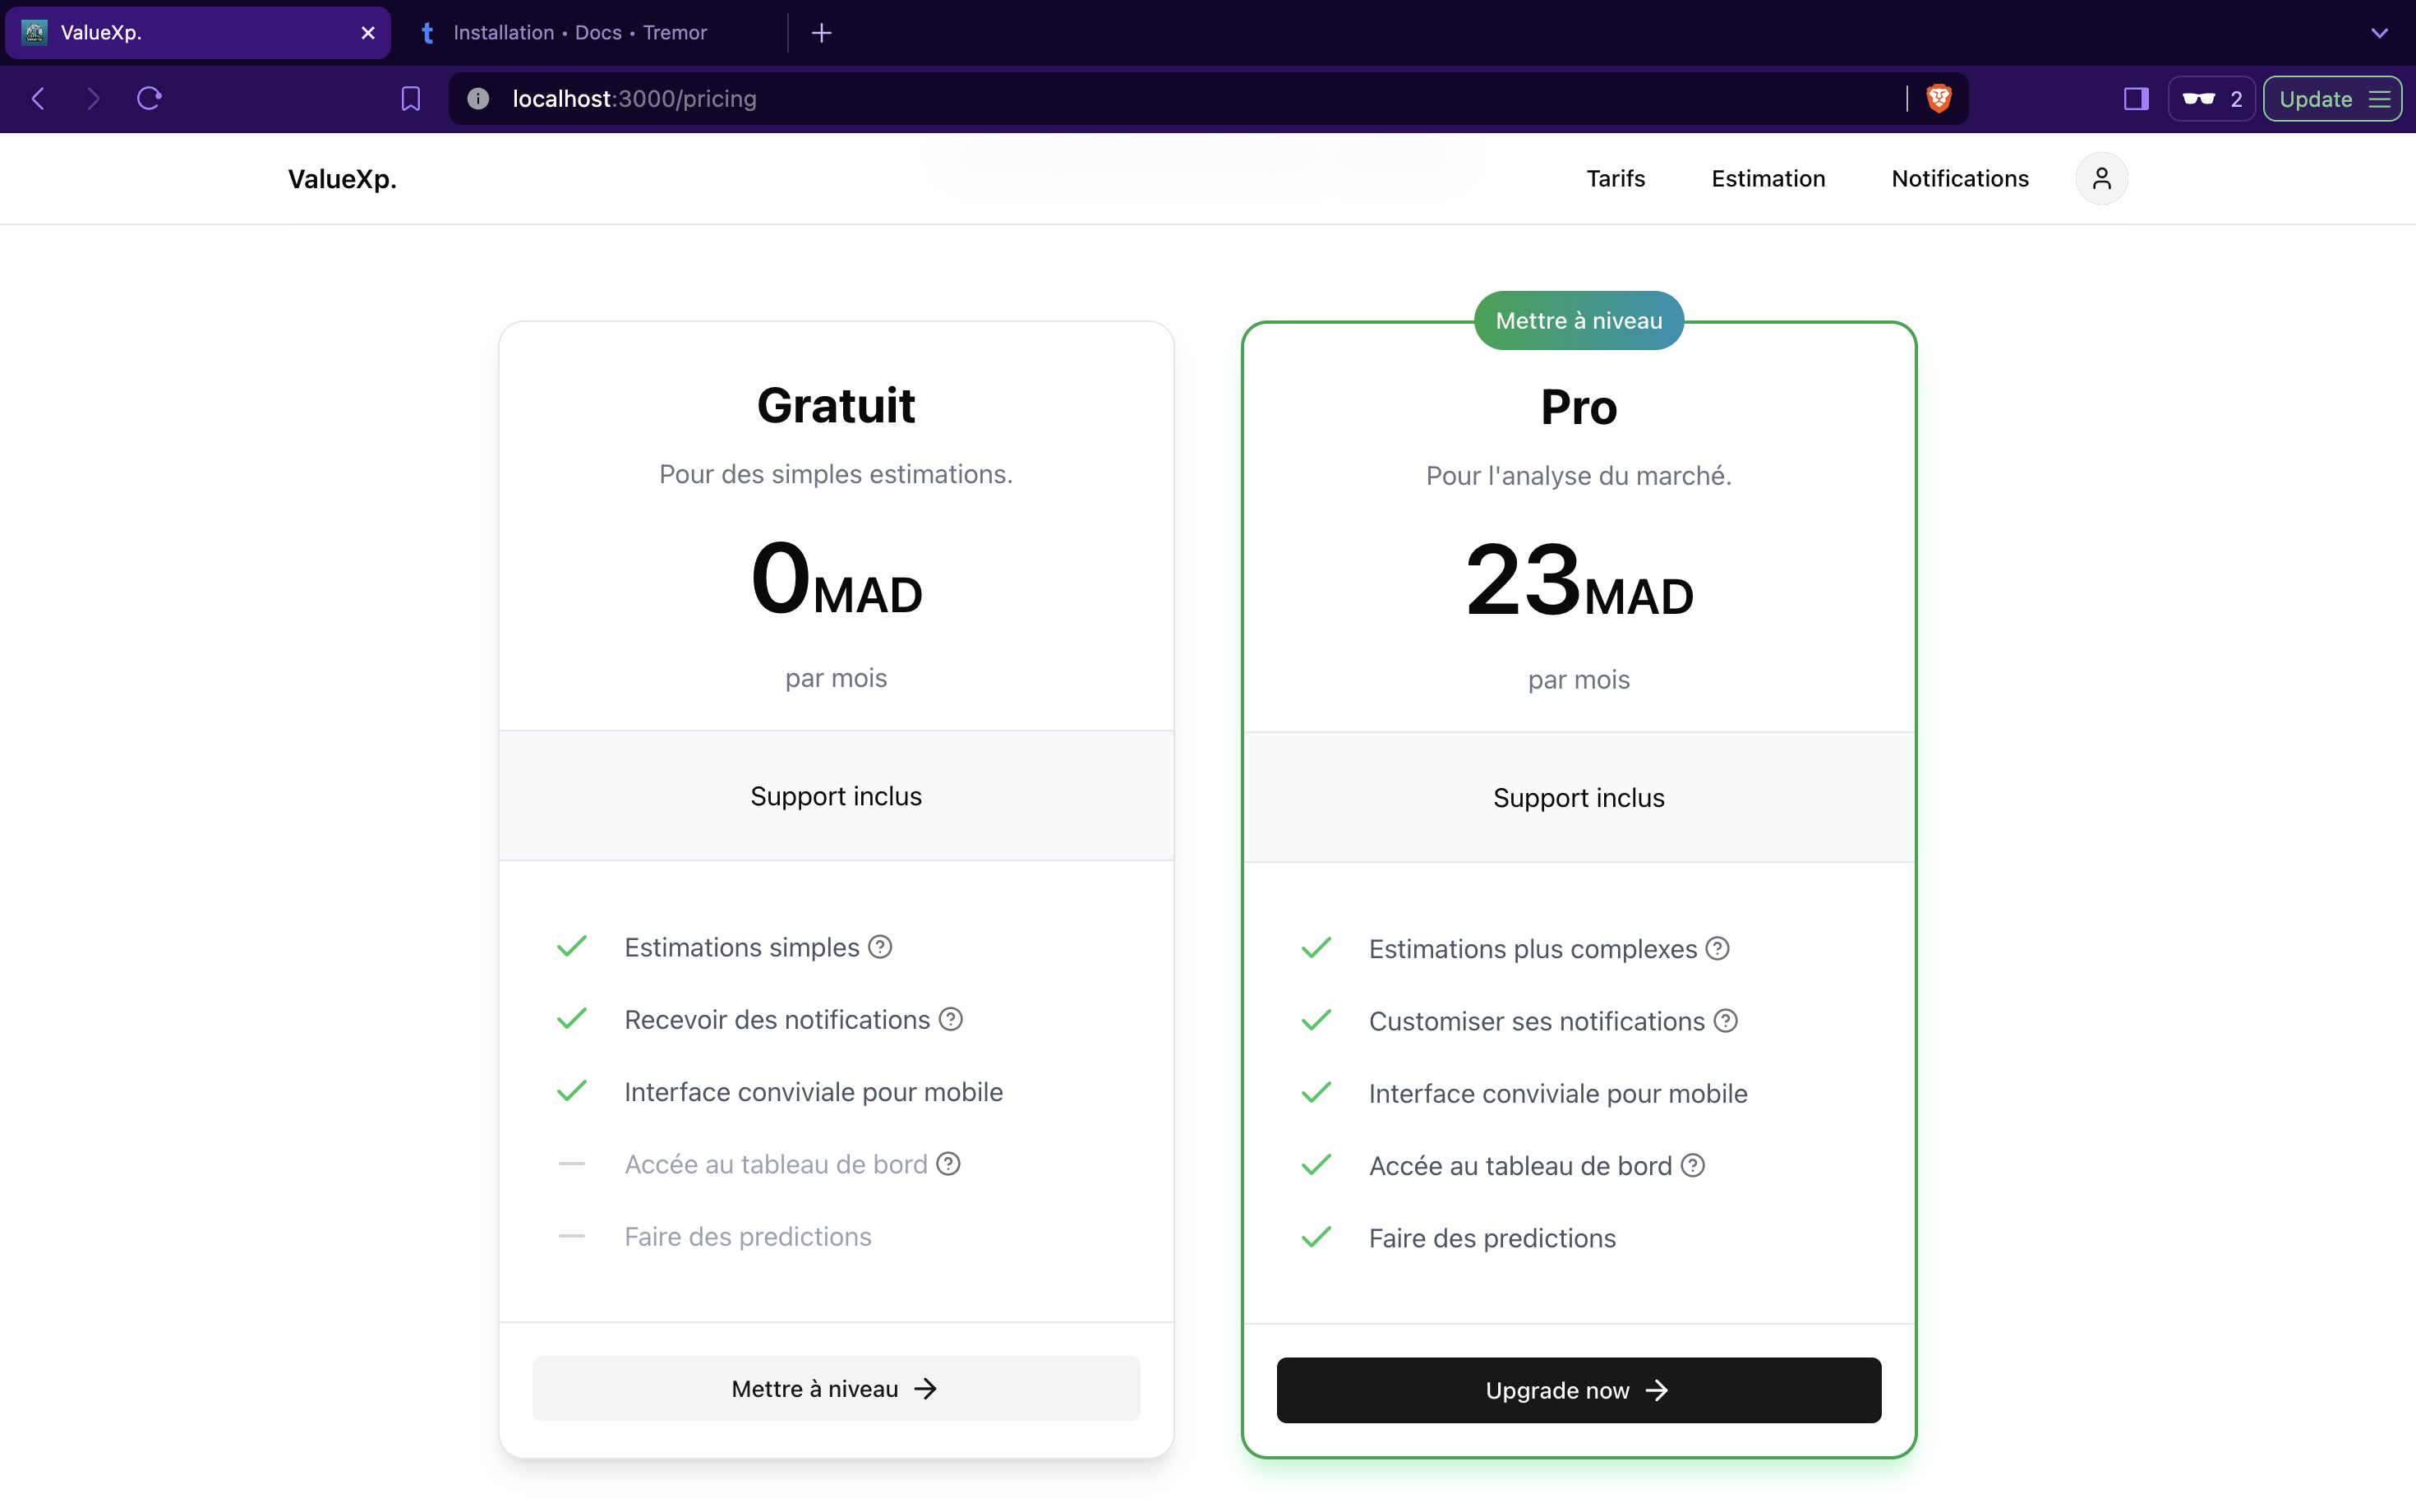
\includegraphics[width=0.9\textwidth]{screens/pricing.png}
    \caption{page de tarification}
    \label{fig:page de tarification}
\end{figure}
\begin{figure}[H]
    \centering
    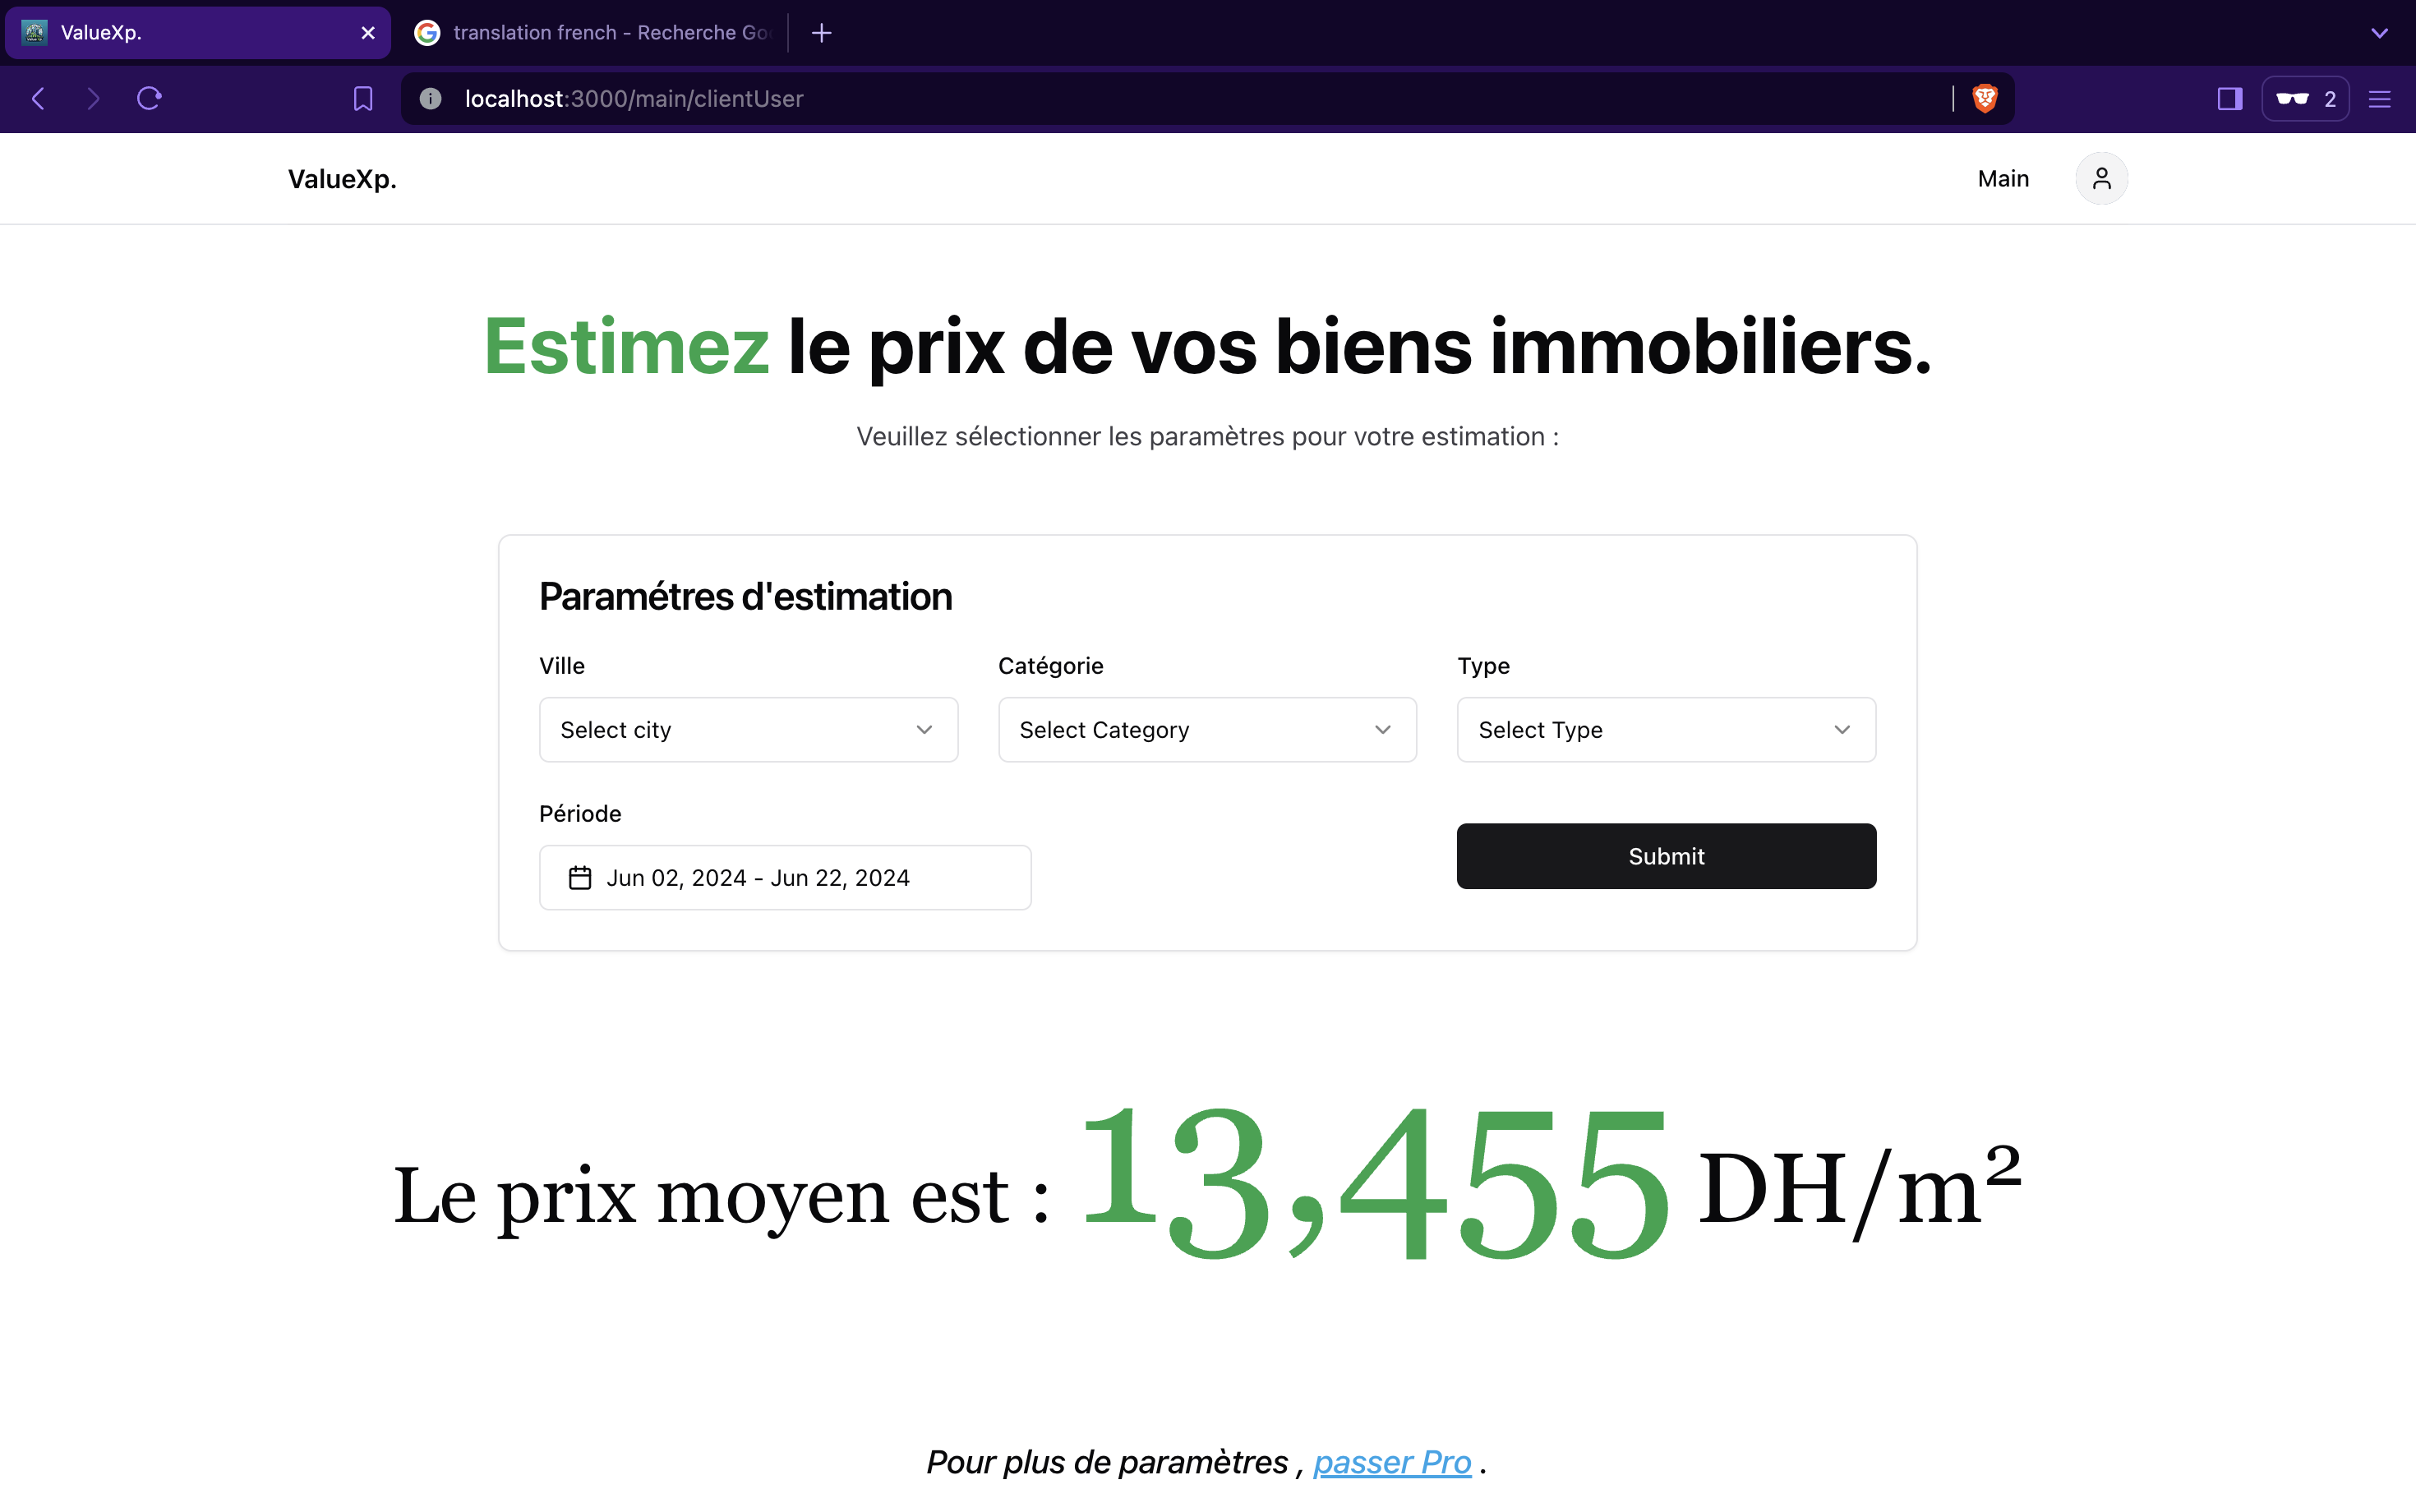
\includegraphics[width=0.6\textwidth]{screens/estimation.png}
    \caption{page d'estimation de prix}
    \label{fig:page d'estimation de prix}
\end{figure}
\begin{figure}[H]
    \centering
    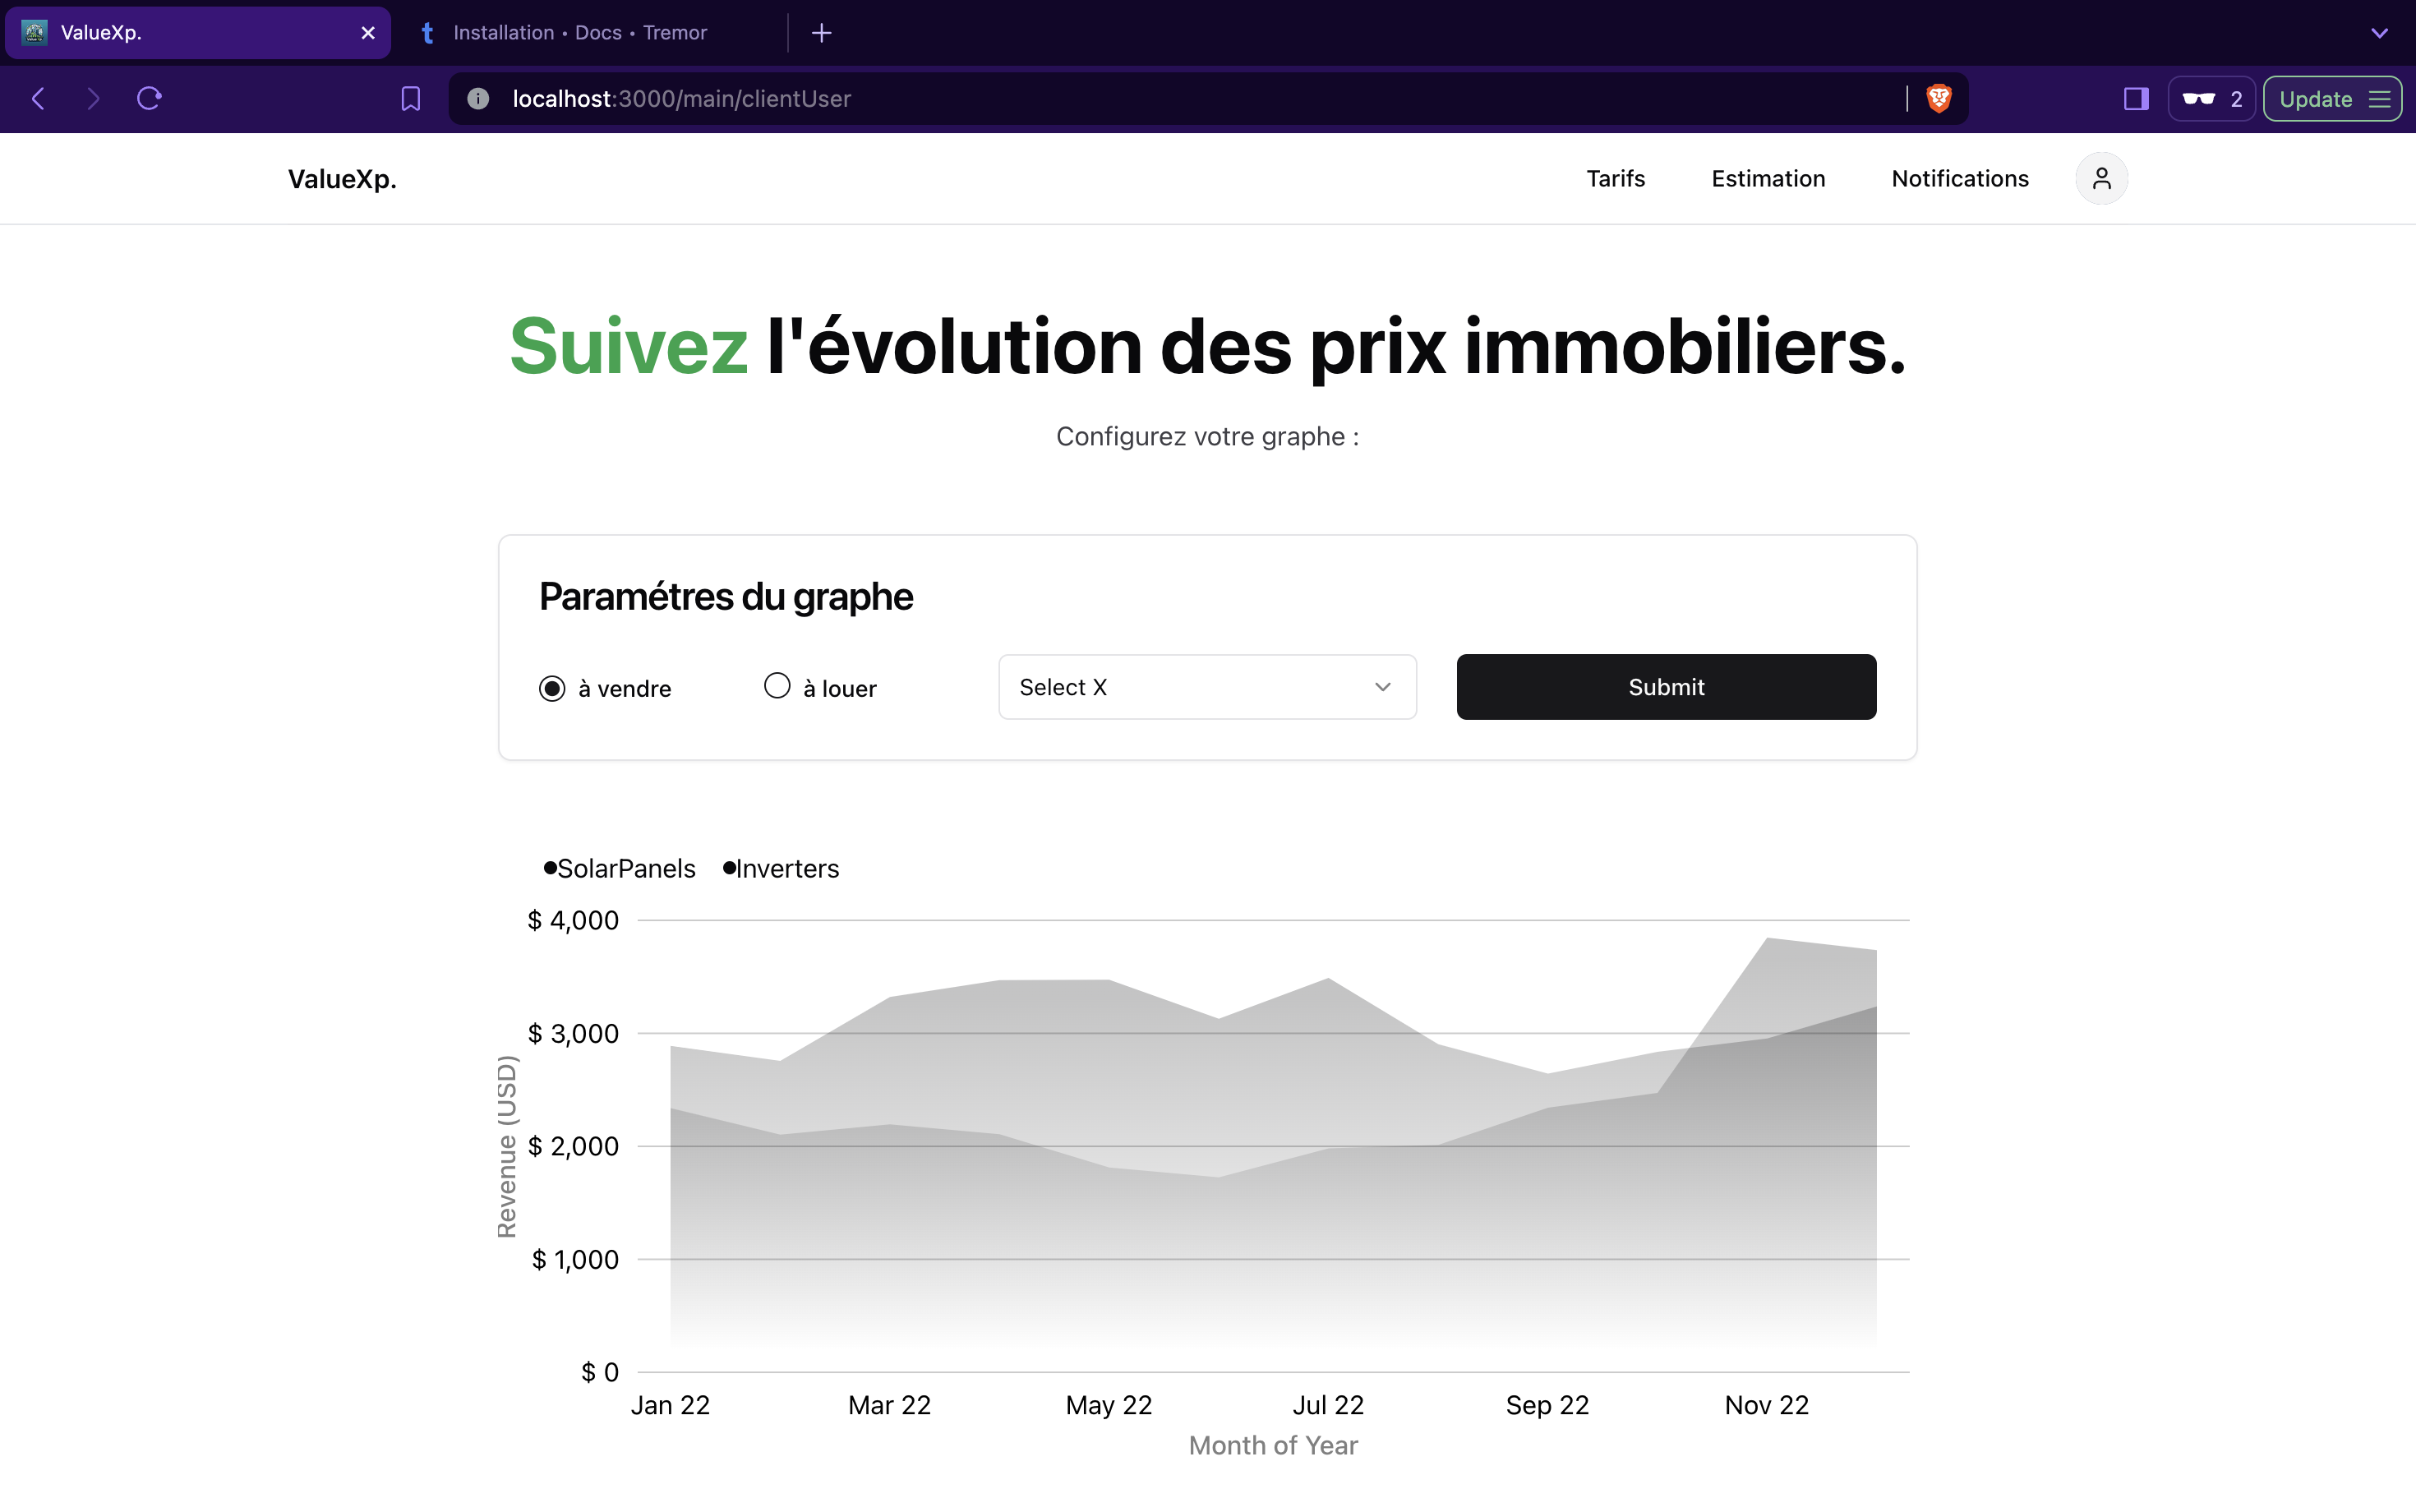
\includegraphics[width=0.6\textwidth]{screens/estimation2.png}
    \caption{page d'évolution des prix}
    \label{fig:page d'évolution des prix}
\end{figure}
\begin{figure}[H]
    \centering
    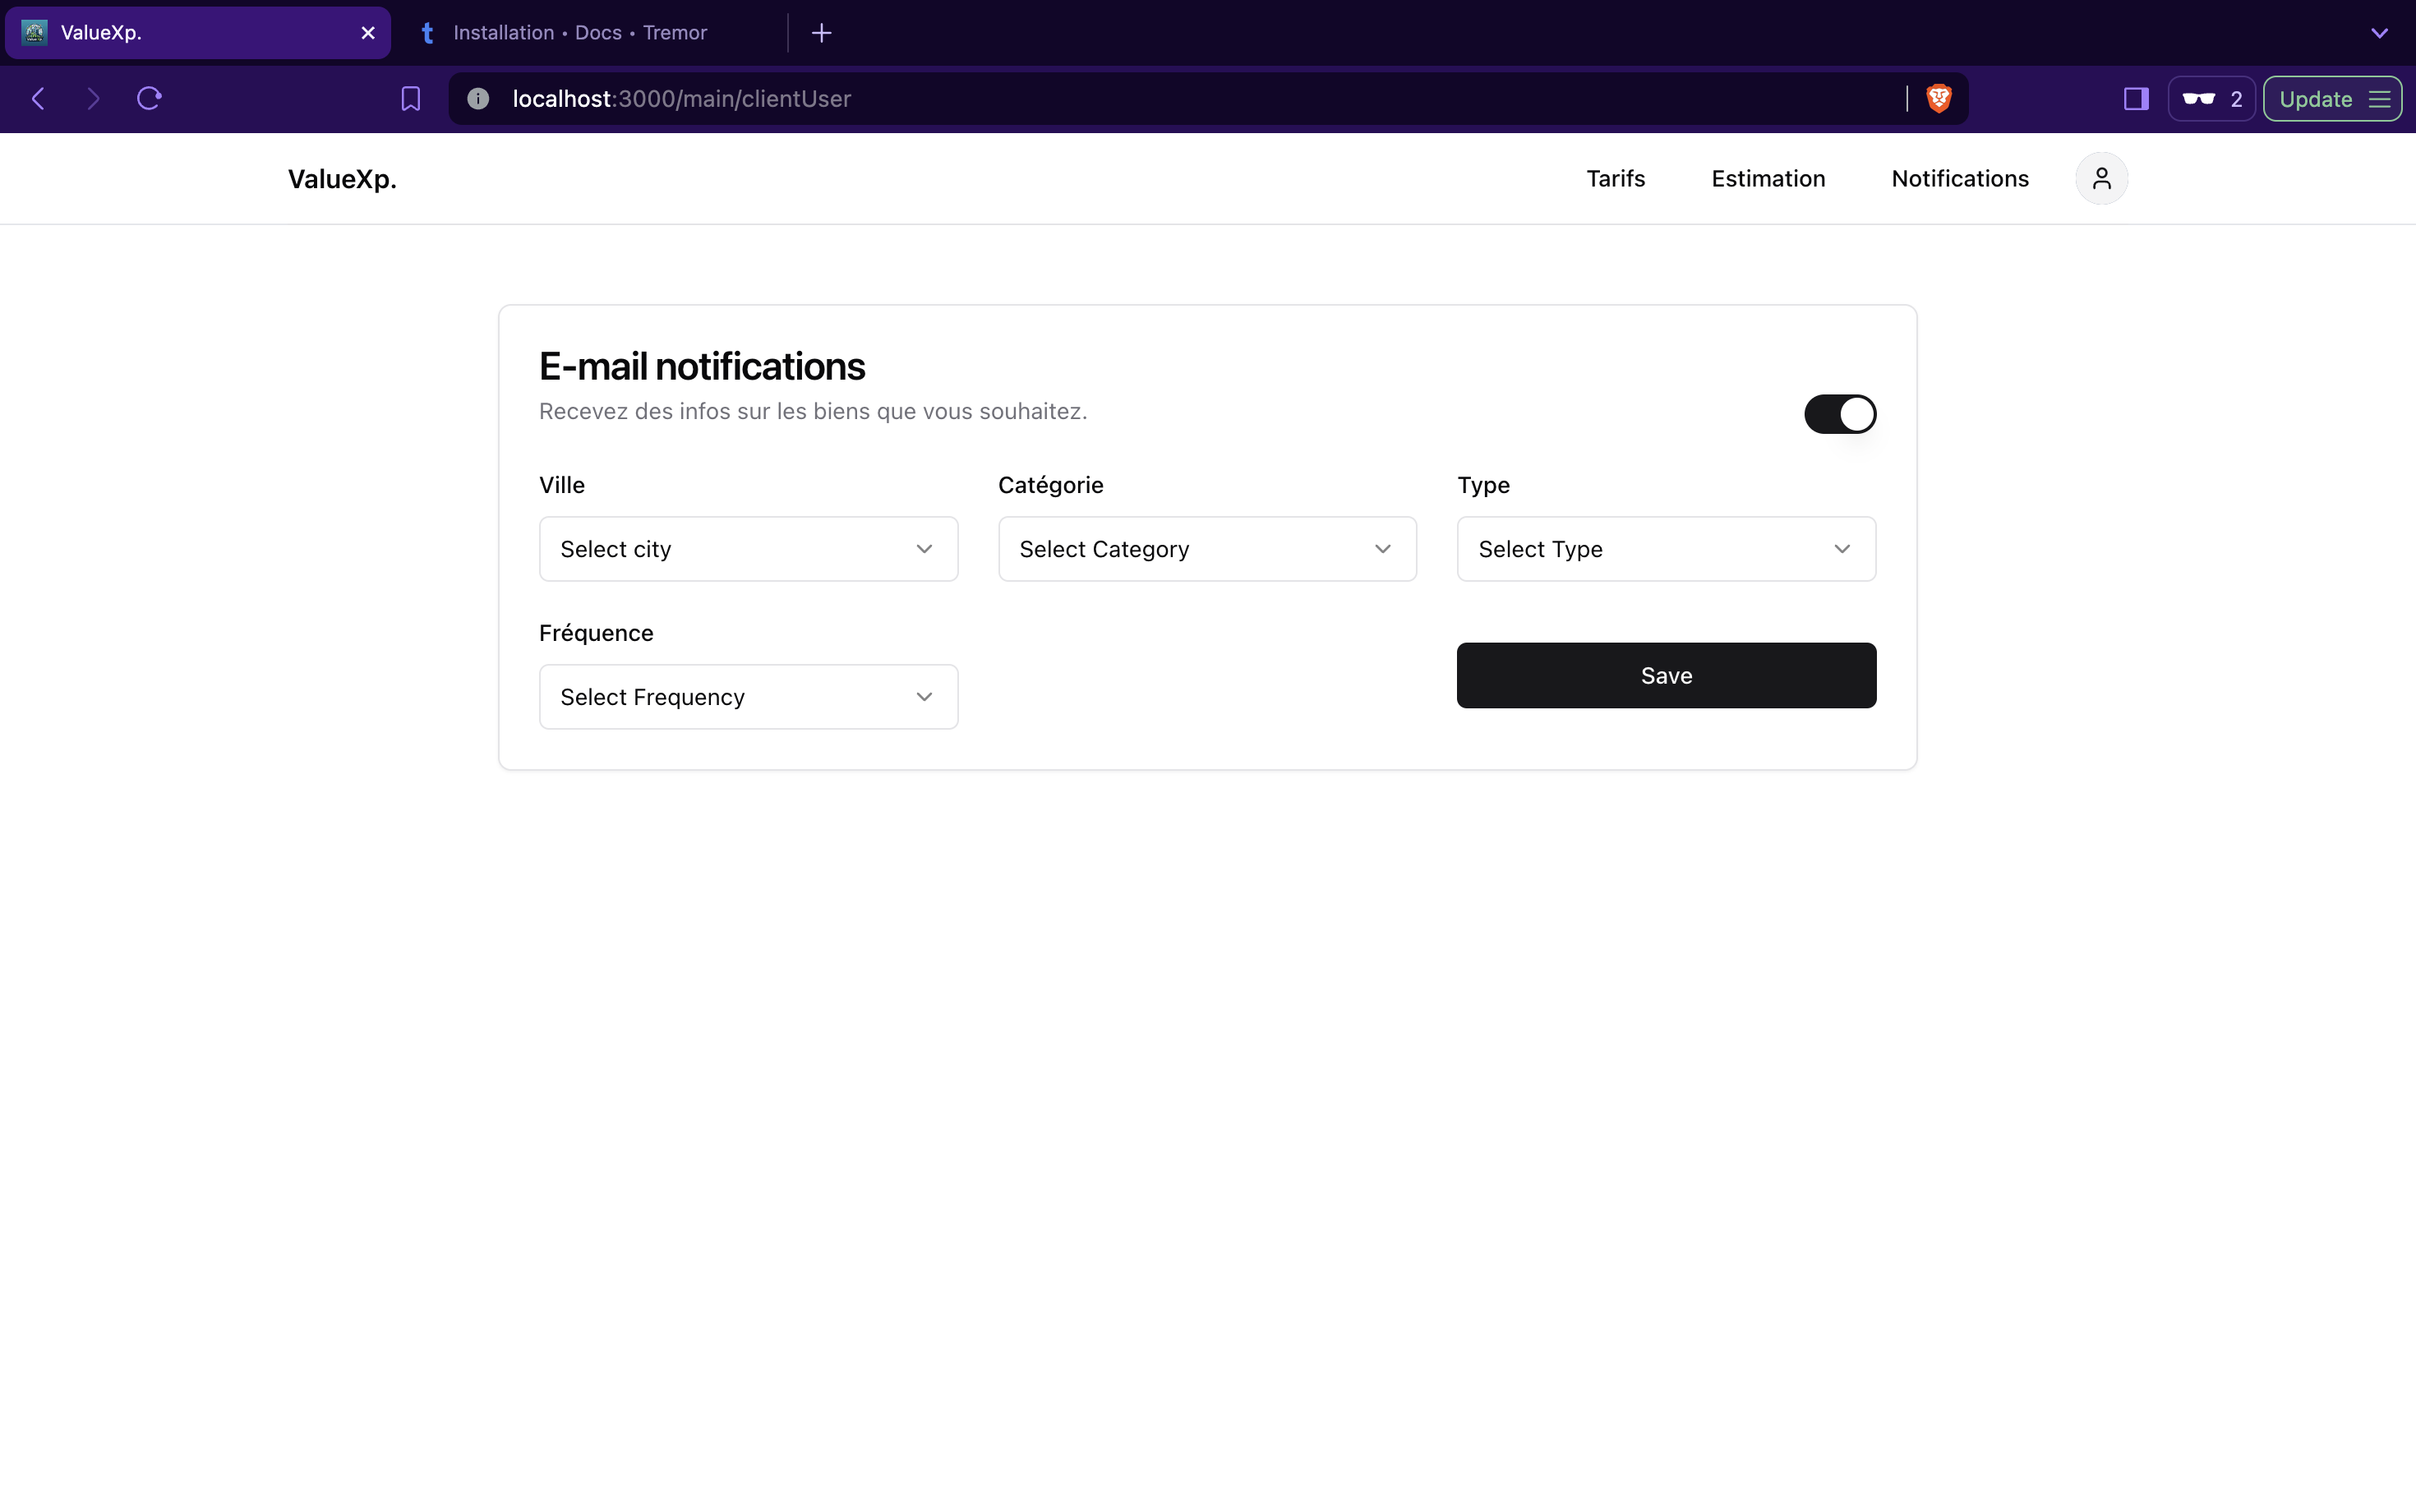
\includegraphics[width=0.6\textwidth]{screens/notif.png}
    \caption{page de notifications}
    \label{fig:page de notifications}
\end{figure}
\end{document}